\documentclass[etd,twoside,senior,noacknowledgments]{BYUPhys}

\usepackage{pdfpages}
\usepackage{listings}
\usepackage[outputdir=out]{minted}
\usepackage{fontspec}
\usepackage{unicode-math}

\setmonofont{Liberation Mono} % needs to be a font that supports unicode characters!

\graphicspath{{./figures}}
\DeclareMathOperator{\J}{J}
\DeclareMathOperator{\struveh}{H}

% Hypergeometric function command (from https://tex.stackexchange.com/a/2477)
\newcommand*\pFqskip{8mu}
\catcode`,\active
\newcommand*\pFq{\begingroup
        \catcode`\,\active
        \def ,{\mskip\pFqskip\relax}%
        \dopFq
}
\catcode`\,12
\def\dopFq#1#2#3#4#5{%
        {}_{#1}F_{#2}\biggl[\genfrac..{0pt}{}{#3}{#4};#5\biggr]%
        \endgroup
}

  \Author{Michael Greenburg}

  \Year{2024}

  \Title{Computationally Modeling Rough Mirrors}

\AdvisorTitle{Advisors}
  \Advisor{Steven Turley, David Allred}

  \Abstract{A program was created to model the effects of surface roughness on reflectance from circular conducting surfaces. Despite tests indicating a correct computational model, ill-conditioned surface impedance matrices mean that the results can't be trusted.}

 \Keywords{mirror, reflect, roughness}

%% The members of your committee (masters only need A and B, PhD need all 4)
%  \MemberA{Committee Member A}
%  \MemberB{Committee Member B}
%  \MemberC{Committee Member C}
%  \MemberD{Committee Member D}
% TODO: do I need any?

\begin{document}

% Start page counting in roman numerals
\frontmatter

% This command makes the formal preliminary pages.
% You can comment it out during the drafting process if you want to save paper.
\makepreliminarypages

% Make the table of contents.
\tableofcontents

% Start regular page counting at page 1
\mainmatter





% INTRO %%%%%%%%%%%%%%%%%%%%%%%%%%%%%%%%%%%%%%%%%%%%%%%%%%%%%%%%%%%%%%%%%%%%%%%%%%%%%%%%%%%%%%%%%%%%%%%%%%%%%%%%%%%%%%%%

\chapter{Introduction} \label{chap:intro}

\section{The Problem} \label{sec:problem}

Modeling reflectance from a conducting surface with roughness that's on the same order of size as the wavelength of incident light is hard \cite{Schroder2011}. The computational model provided here is meant to accurately predict such reflectance.



\section{The Attempted Solution} \label{sec:attempted_solution}

A \href{https://github.com/mjg0/Mirrors.jl}{Julia package} was written to calculate the far-field reflectance from a rough circular conducting mirror using the model below [\ref{chap:methods}]. It's available as in appendix \ref{chap:julia} and on GitHub at https://github.com/mjg0/Mirrors.jl.



\section{Note on Plots} \label{sec:plots_note}

Two types of plots will be used frequently here: plots of mirrors and plots of reflectance. Mirror plots are what one would expect: the mentioned parameter (e.g. height, electric field) is mapped on the shape of the mirror itself. Reflectance plots are \href{https://en.wikipedia.org/wiki/Azimuthal_equidistant_projection}{polar azimuthal equidistant projections} centered at normal to the mirror and extending to 90 degrees, much like a map of the northern hemisphere centered at the North Pole and extending to the equator, with the magnitude of reflected light corresponding to the intensity of the color.

%%%%%%%%%%%%%%%%%%%%%%%%%%%%%%%%%%%%%%%%%%%%%%%%%%%%%%%%%%%%%%%%%%%%%%%%%%%%%%%%%%%%%%%%%%%%%%%%%%%%%%%%%%%%%%%%%%%%%%%%





% EXPECTED RESULTS %%%%%%%%%%%%%%%%%%%%%%%%%%%%%%%%%%%%%%%%%%%%%%%%%%%%%%%%%%%%%%%%%%%%%%%%%%%%%%%%%%%%%%%%%%%%%%%%%%%%%

\chapter{Methods} \label{chap:methods}

\section{Modeling Expected Results} \label{sec:expected_results}

It's vital to ensure that the program can correctly predict reflectance for a flat mirror--failing that, it can't be trusted to predict reflectance for rough surfaces. We thus need an equation that can predict far-field reflectance for an ideal mirror given an incident beam angle. Physical optics are used for simplicity.

\subsection{Huygens Approximation} \label{subsec:huygens_approx}

Since a finite, perfectly reflective surface is analogous to an aperture, the Huygens-Fresnel principle is used to approximate the behavior of circular mirrors. An easy test of the approximation will be its results when light strikes from normal to the surface: it should be proportional to the Airy pattern:

\begin{equation}\label{eq:airy}
  \frac{\J_1(kR\sin(\theta))}{kR\sin(\theta)}
\end{equation}

\ldots where $k$ is the wave number, $\frac{2\pi}{\lambda}$ ($\lambda$ being the wavelength), $R$ is the radius of the aperture (mirror in our case), and $\theta$ is the angle at which the reflectance is measured. $J_1$ is the first order Bessel function of the first kind.

\subsection{Setup} \label{sec:setup}

The electric field on a flat mirror in the x-y plane due to a plane wave coming in at an angle $\alpha$ from normal (the z axis), inclined toward the x axis, is proportional to:

\begin{equation}
  e^{ikx\sin\left({\alpha}\right)}
\end{equation}

The contribution of one point on the mirror to the far field reflectance at some polar angle $\theta$ and azimuthal angle $\phi$ is that exponential multiplied by some phase shift.

\subsection{Phase Shift} \label{sec:phase_shift}

The phase shift relative to the origin suffices since far-field reflectance is sought. For some point $p$, the distance $d$ between that point and the origin \textit{along the direction of travel toward the point in the far field} defined by $\theta$ and $\phi$ is needed.

\begin{figure}
  \centerline{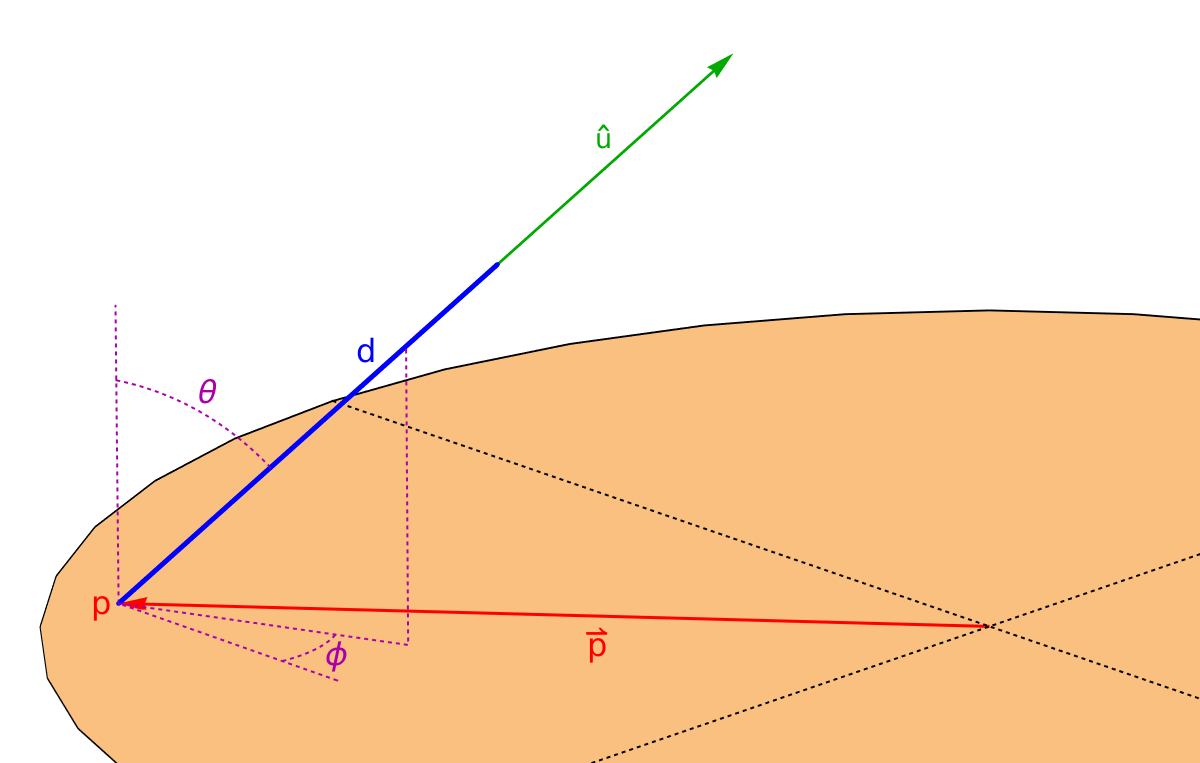
\includegraphics[width=\textwidth]{phase-length}}
  \caption[Phase length of a beam of light]{\label{fig:phase_length}
    $d$ is the phase shift of light coming from $p$ relative to light coming from the origin.}
\end{figure}

$d$ is given by dotting the unit vector $\hat{u}$ with $-\vec{p}$ [\ref{fig:phase_length}]. $\hat{u}$ is $\left(\sin{\theta}\cos{\phi},\sin{\theta}\sin{\phi},\cos{\theta}\right)$, so $d$ is:

\begin{equation}
  -x_p\sin{\theta}\cos{\phi}-y_p\sin{\theta}\sin{\phi}
\end{equation}

\ldots where $x_p$ and $y_p$ are the $x$ and $y$ coordinates of $p$.

The corresponding phase shift is thus:

\begin{equation}
  e^{-ik(x_p\sin{\theta}\cos{\phi}+y_p\sin{\theta}\sin{\phi})}
\end{equation}

\ldots so the contribution to the far field by a given point is:

\begin{equation}
  e^{ikx\sin\left({\alpha}\right)}e^{-ik(x_p\sin{\theta}\cos{\phi}+y_p\sin{\theta}\sin{\phi})}
\end{equation}

\ldots or:

\begin{equation}
  e^{ik\left(x_p(\sin{\alpha}-\sin{\theta}\cos{\phi})-y_p\sin{\theta}\sin{\phi}\right)}
\end{equation}

For simplicity, $a$ and $b$ are defined as:

\begin{equation}
  a = k\left(\sin{\alpha}-\sin{\theta}\cos{\phi}\right)
\end{equation}
\begin{equation}
  b = -k\sin{\theta}\sin{\phi}
\end{equation}

\ldots so that the contribution from $p$ to the far field can be represented as:

\begin{equation}
  e^{i(ax_p+by_p)}
\end{equation}

\subsection{Integrating} \label{sec:integrating}

To find the total contribution to the far field from the entire mirror (of radius $R$) at some $\theta$ and $\phi$, this contribution must be integrated over the entire surface:

\begin{equation}\label{eq:integral1}
  \int_0^{2\pi}\int_0^R e^{i(ar\cos(\Theta)+br\sin(\Theta))} rdrd\Theta
\end{equation}

\ldots where $r\cos\Theta$ and $r\sin\Theta$ have been substituted for $x$ and $y$ respectively.

The solution (see appendix \ref{chap:integral}) is:

\begin{equation}\label{eq:expected_refl}
  \pi R^2 \pFq{0}{1}{}{2}{-\frac{R^2}{4}\left(a^2+b^2\right)}
\end{equation}

\ldots where ${}_0 F_1$ is the confluent hypergeometric limit function. Subbing $a$ and $b$ back in appropriately, and using $\frac{2\pi}{\lambda}$ in $k$'s stead, gives:

\begin{equation}
  \pi R^2 \pFq{0}{1}{}{2}{-\frac{\pi^2 R^2}{\lambda^2}\left(\sin^2\alpha+\sin^2\theta-2\sin\alpha\sin\theta\cos\phi\right)}
\end{equation}

As a quick check, when $\alpha$ is 0 (indicating normal incident light), this is proportional to equation \ref{eq:airy} as it should be (see appendix \ref{chap:airy_validation}).

%%%%%%%%%%%%%%%%%%%%%%%%%%%%%%%%%%%%%%%%%%%%%%%%%%%%%%%%%%%%%%%%%%%%%%%%%%%%%%%%%%%%%%%%%%%%%%%%%%%%%%%%%%%%%%%%%%%%%%%%





% MIRROR MODELING %%%%%%%%%%%%%%%%%%%%%%%%%%%%%%%%%%%%%%%%%%%%%%%%%%%%%%%%%%%%%%%%%%%%%%%%%%%%%%%%%%%%%%%%%%%%%%%%%%%%%%

\section{Mirror Modeling} \label{section:mirror_modeling}

The simulated mirror is a circle broken up into rings of equal annular width $a$, each broken into patches of equal area $\frac{\pi a^2}{3}$. The first ring is broken into 3 patches, the second into 9, etc.; ring $n$ has $6n+3$ patches, and a mirror of $N$ rings has $3N^2$ total patches. Each patch has four points placed at:

\begin{equation}
  r = a \left(\frac{2n+1}{2} \pm \frac{1}{2\sqrt{3}}\right)
\end{equation}
\begin{equation}
  \theta = 2\pi \left(\frac{2m+1}{12n+6} \pm \frac{1}{\left(12n+6\right)\sqrt{3}}\right)
\end{equation}

\ldots where $n$ is the ring index (starting from 0 at the center of the mirror) and $m$ is the patch index (starting at 0 and going to $6n-2$). The height $z$ at each point varies based on the mirror's roughness. See figure \ref{fig:patches_points} for an illustration.

This spacing was chosen since it gives a fourth order error term [\ref{chap:circular_integration}].

\begin{figure}
  \centerline{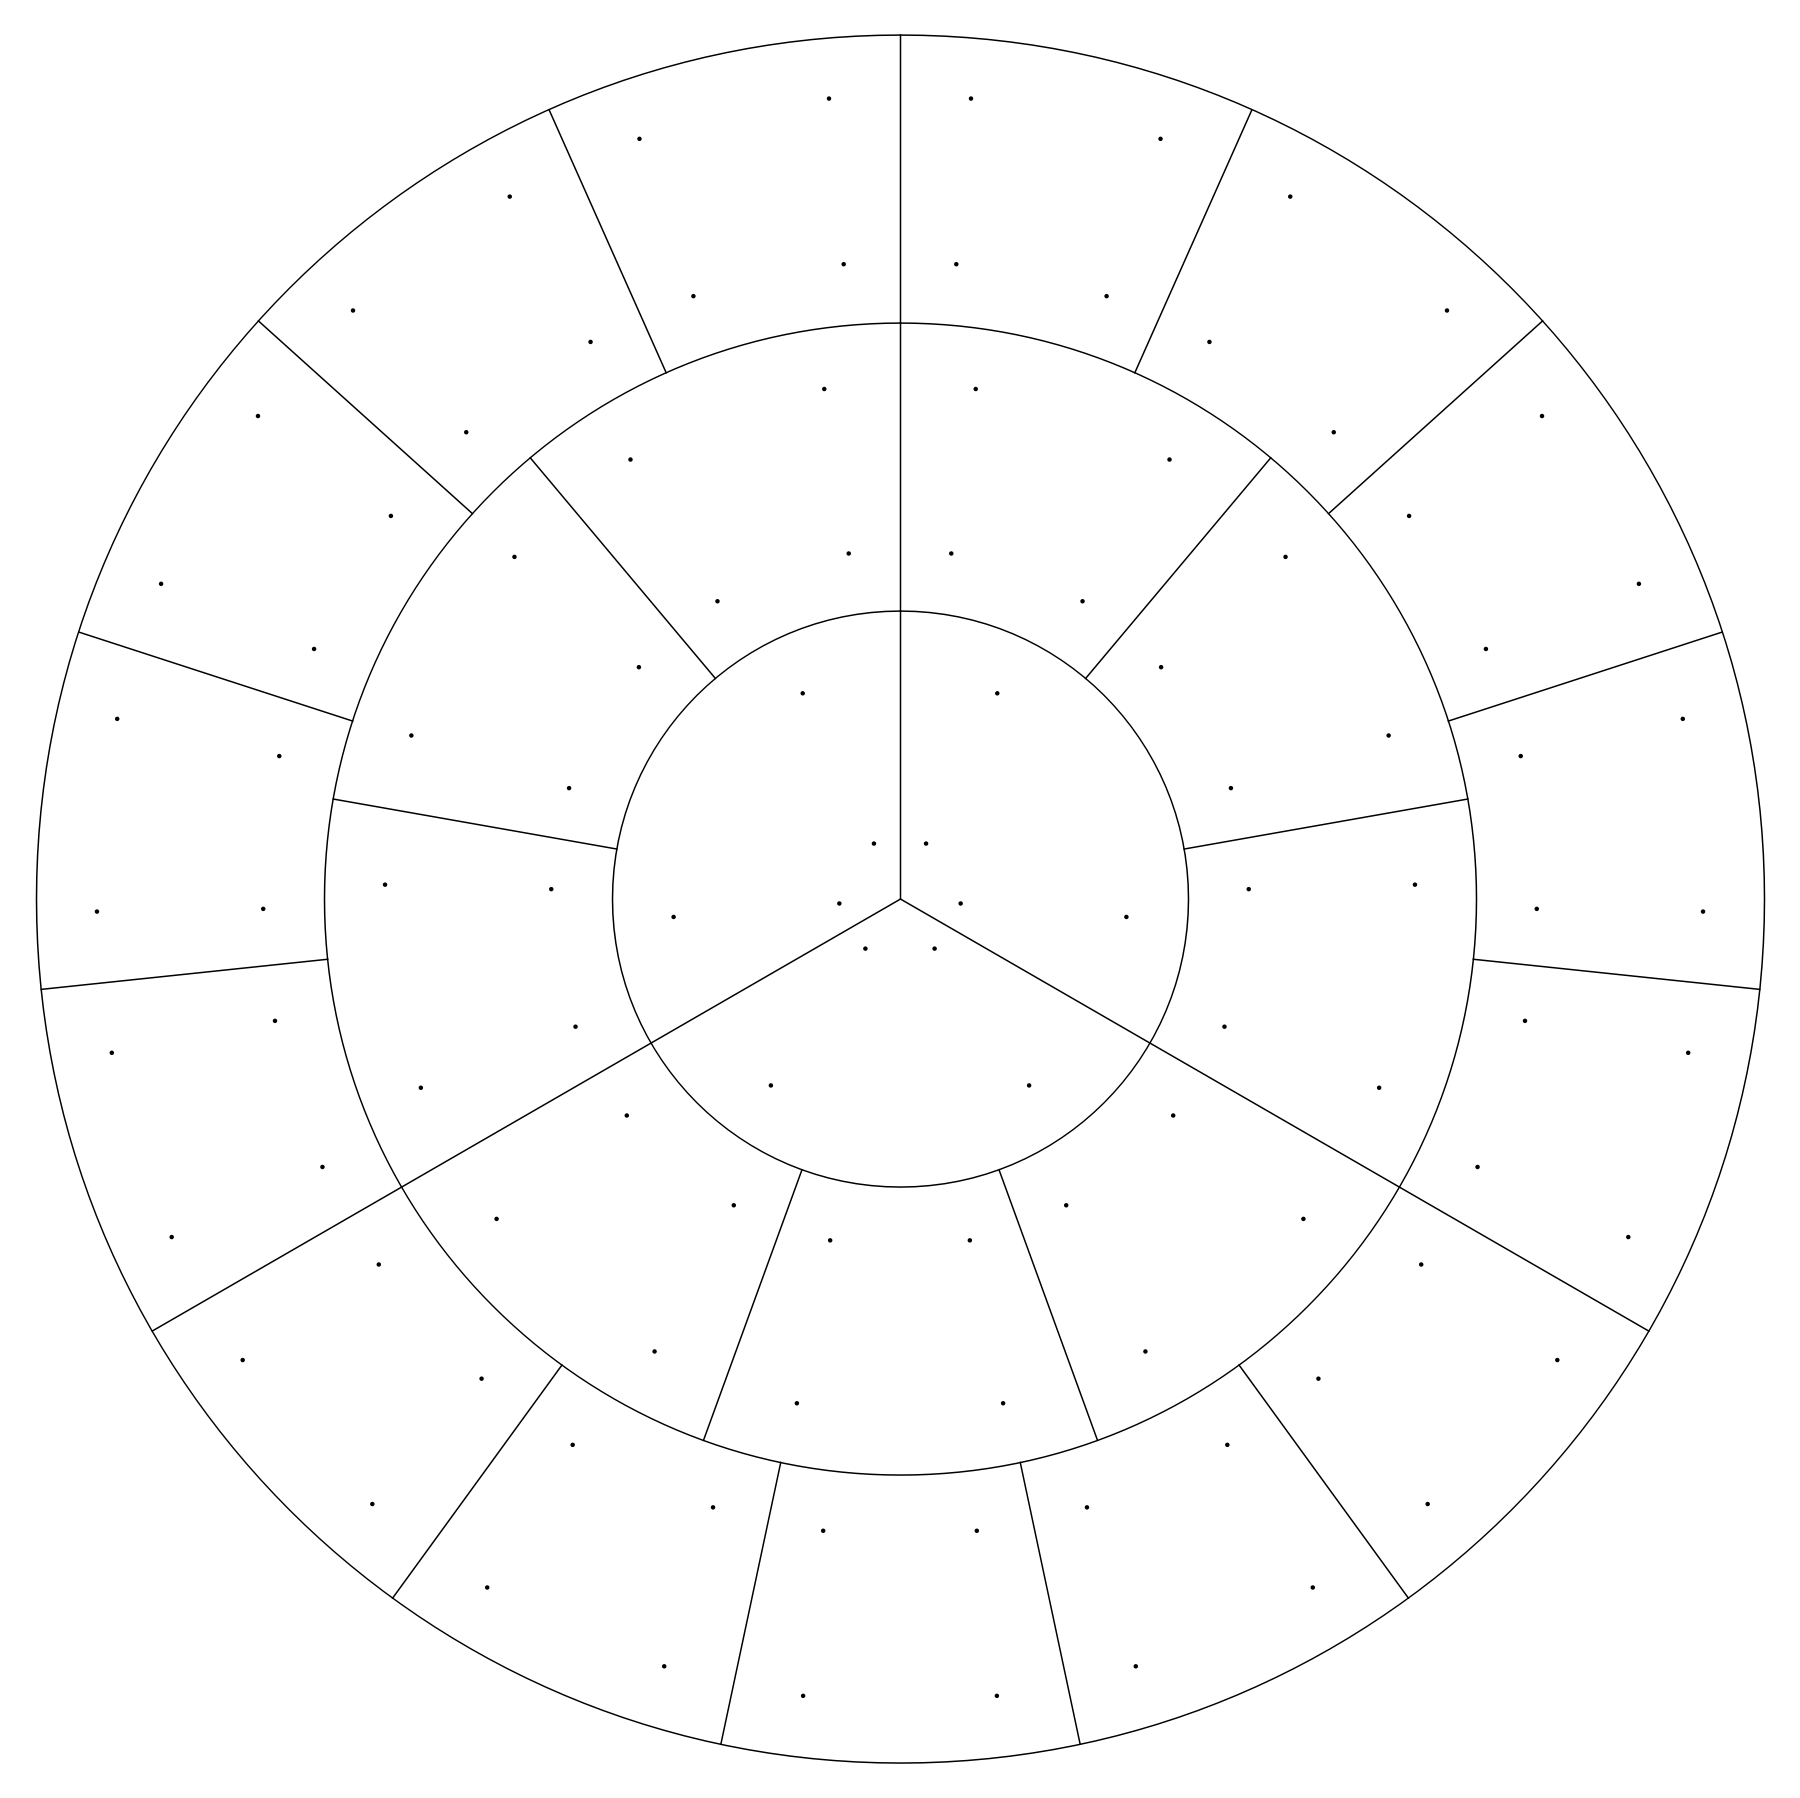
\includegraphics[width=\textwidth]{circular-grid-with-points}}
  \caption[Mirror patch boundaries and point locations]{\label{fig:patches_points}
    The patch boundaries and points of a mirror with 3 rings.}
\end{figure}



\section{Electric Field at Surface}\label{chap:efield}

At each of the points on the mirror the electric field is calculated as follows, assuming a plane wave of wavelenth $\lambda$ coming in at angle $\alpha$ from normal (direction of $z$) in the x-y plane:

\begin{equation}
  k_{x}=2\pi\lambda\cos\left(\alpha\right)
\end{equation}

\begin{equation}
  k_{z}=-2\pi\lambda\sin\left(\alpha\right)
\end{equation}

\begin{equation}
  E_{pt}=e^{i\left(k_{x}x+k_{z}z\right)}
\end{equation}



\section{Impedance Matrix} \label{sec:impedance}

The impedance matrix is a square matrix whose length along each axis is the number of points on the surface. There are two main sections, the part representing the interaction between different patches and the part representing the interaction of a patch with itself. The same-patch portion of the matrix consists of the 4x4 blocks along the main diagonal (one block for each patch), and the different-patch portion is the remainder.

\subsection{Different patch} \label{sec:different_patch}

Since there's no chance of hitting a singularity when computing how two different patches interact, each non-singular interaction for points $i$ and $j$ can be calculated with:

\begin{equation}
  Z_{i,j}=\frac{\pi a}{12n_{j}+6}G\left(p_{i},p_{j}\right)r_{j}
\end{equation}

...where the first fraction is a Jacobian (see Circular Integration [\ref{chap:circular_integration}] equation 22--I've subbed in $r_{j}$ for $a\left(n+\frac{1}{2}+\frac{1}{2\sqrt{3}}\right)$) and $G$ is the Green's function.

\subsection{Same patch} \label{sec:same_patch}

This is harder due to the need to deal with singularities. In essence, each annular patch is transformed into a square, then split into 4 triangles with a common vertex at the point in question, then that point stretch into a line to turn each triangle into a square over which to integrate, reducing the order of the singularity. For numerical convenience, the triangular portion of the patch is turned into a square bounded by $(0,0)$ to $(1,1)$. Then a function of two variables, $u$ and $v$ below, can be integrated over this square (see Circular Integration [\ref{chap:circular_integration}] sections 5.6 and 5.7):

\begin{equation}
  r\left(u,v\right)=B_{2,1}u+B_{2,2}uv\pm\frac{a}{2\sqrt{3}}+a\left(n+\frac{1}{2}\right)
\end{equation}

\begin{equation}
  \theta\left(u,v\right)=\frac{2\pi}{a(6n+3)}\left(a\left(m+\frac{1}{2}\right)+B_{1,1}u+B_{1,2}uv\pm\frac{a}{2\sqrt{3}}\right)
\end{equation}

...where $B$ is a matrix that allows transformation between a triangular piece of an annular patch and a square; in all there are 16 $B$ matrices, for 4 points with 4 corresponding triangles each (see Circular Integration [\ref{chap:circular_integration}] subsection 5.5.1).

It's easy enough to get a function of $u$ and $v$ from the function of $r$, $\theta$, and $z$ to be integrated:

\begin{equation}
  f\left(u,v\right)=f\left(r\left(u,v\right),\theta\left(u,v\right),z\left(r\left(u,v\right),\theta\left(u,v\right)\right)\right)
\end{equation}

For utility a transform function is defined, taking a point ($r$, $\theta$, and $z$, with associated $n$ and $p$) and a function of that point, and yielding a function of $u$ and $v$:

\begin{equation}
  T\left(f,p\right)=\left(u,v\right)\rightarrow r\left(u,v\right)f\left(u,v\right)
\end{equation}

With this transform function, the integral of a function $f$ over a patch for a certain point $p$ can be calculated:

\begin{equation}
  P\left(f,p\right)=\frac{2\pi}{a\left(6n+3\right)}\sum_{triangles}|det\left(B_{t}\right))|H\left(T\left(f,p\right)\right)_{0,0}^{1,1}
\end{equation}

\ldots where $H$ is \texttt{HCubature} \cite{HCubature}.

The desired function is the Green's function of the point with another point:

\begin{equation} \label{eq:greens}
  G\left(p_{1},p_{2}\right)=\frac{e^{ik\rho}}{4\pi\rho}
\end{equation}

...where $k$ is the wave number and $\rho$ is the distance between the two points. The point to be integrated around can be fixed (since $P$ requires a function of one point) and the resultant function called $G^{*}\left(p_{2}\right)$.

This function can then be used to determine the elements of the 4x4 block representing this patch's interaction with itself (see Circular Integration [\ref{chap:circular_integration}] section 6.1):

\begin{equation}
  K_{1}=P\left(G^{*},p\right)
\end{equation}

\begin{equation}
  K_{2}=P\left(G^{*}x_{p},p\right)
\end{equation}

\begin{equation}
  K_{3}=P\left(G^{*}y_{p},p\right)
\end{equation}

\begin{equation}
  K_{4}=P\left(G^{*}x_{p}y_{p},p\right)
\end{equation}

One row of the 4x4 block is thus:

\begin{equation}
  Z_{s,s'}=\frac{K_{1}}{4}+\frac{\sqrt{3}}{2a}\left(-K_{2}-K_{3}\right)+\frac{3}{a^{2}}K_{4}
\end{equation}

\begin{equation}
  Z_{s,s'+1}=\frac{K_{1}}{4}+\frac{\sqrt{3}}{2a}\left(-K_{2}+K_{3}\right)-\frac{3}{a^{2}}K_{4}
\end{equation}

\begin{equation}
  Z_{s,s'+2}=\frac{K_{1}}{4}+\frac{\sqrt{3}}{2a}\left(K_{2}+K_{3}\right)+\frac{3}{a^{2}}K_{4}
\end{equation}

\begin{equation}
  Z_{s,s'+3}=\frac{K_{1}}{4}+\frac{\sqrt{3}}{2a}\left(K_{2}-K_{3}\right)-\frac{3}{a^{2}}K_{4}
\end{equation}

\ldots where $s$ is the index of this point ($p$) and $s'$ is the first index of the other patch.

%%%%%%%%%%%%%%%%%%%%%%%%%%%%%%%%%%%%%%%%%%%%%%%%%%%%%%%%%%%%%%%%%%%%%%%%%%%%%%%%%%%%%%%%%%%%%%%%%%%%%%%%%%%%%%%%%%%%%%%%





% REFLECTANCE %%%%%%%%%%%%%%%%%%%%%%%%%%%%%%%%%%%%%%%%%%%%%%%%%%%%%%%%%%%%%%%%%%%%%%%%%%%%%%%%%%%%%%%%%%%%%%%%%%%%%%%%%%

\section{Surface Current} \label{sec:current}

Since $Z \times E = J$ (where $Z$ is the impedance matrix, $E$ is the electric field, and $J$ is the surface current), once $Z$ and $E$ are determined $J$ can be computed as $Z\\E$. See Circular Integration section 6 (appendix \ref{chap:circular_integration}).



\section{Reflectance} \label{sec:reflectance}

Given $J$, reflectance for a given $\theta$ (polar) and $\phi$ (azimuthal) is determined by:

\begin{equation}
  R=\sum_{pts}J_{pt}e^{-ik\left(x\sin\left(\theta\right)\cos\left(\phi\right)+y\sin\left(\theta\right)\cos\left(\phi\right)+z\cos\left(\theta\right)\right)}
\end{equation}

The real part squared gives us the intensity at infinity for a certain angle.

%%%%%%%%%%%%%%%%%%%%%%%%%%%%%%%%%%%%%%%%%%%%%%%%%%%%%%%%%%%%%%%%%%%%%%%%%%%%%%%%%%%%%%%%%%%%%%%%%%%%%%%%%%%%%%%%%%%%%%%%





% CODE %%%%%%%%%%%%%%%%%%%%%%%%%%%%%%%%%%%%%%%%%%%%%%%%%%%%%%%%%%%%%%%%%%%%%%%%%%%%%%%%%%%%%%%%%%%%%%%%%%%%%%%%%%%%%%%%%

\section{The Code}\label{sec:code}

The Julia package \href{https://github.com/mjg0/Mirrors.jl}{Mirrors.jl} (which is included as an appendix [\ref{chap:julia}]) was built and used for computation. Here's an example of its usage:

\begin{minted}{julia}
  using Mirrors, Plots

  # Create a Mirror object
  radius = 2.5 # units are wavelengths
  N = 20       # number of rings
  rms = 0.0    # RMS of surface roughness (wavelengths)
  sigma = 0.0  # stdev of surface roughness (wavelengths)
  M = Mirror(radius, N, rms, sigma)

  # Find the mirror's impedance
  Z = impedance(M)

  # Find the electric field induced by a uniform plane wave
  alpha = pi/8 # incident beam angle
  E = electricfield(M, alpha)

  # Find the surface current due to E
  J = Z \ E

  # Determine and plot reflectance
  R = Reflectance(M, J)
  heatmap(R)
\end{minted}

The resultant heatmap, with a few extra parameters for the \texttt{heatmap} call [\ref{chap:heatmap_code}], might look like figure \ref{fig:sample_heatmap}.

\begin{figure}
  \centerline{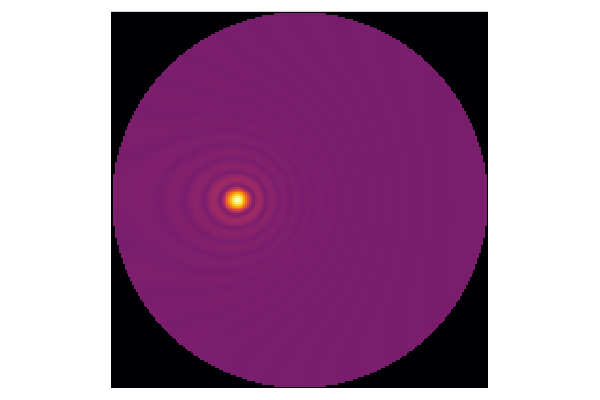
\includegraphics[width=.7\textwidth]{sample-reflectance}}
  \centerline{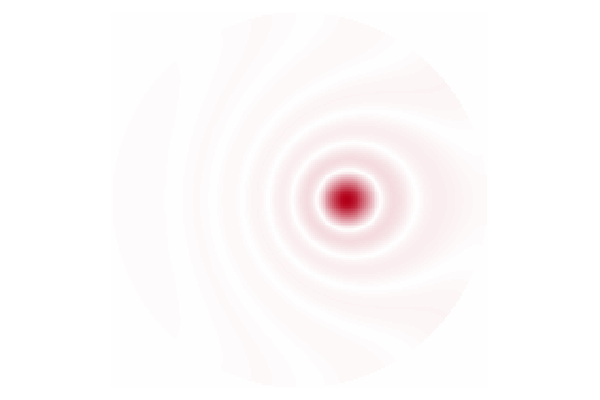
\includegraphics[width=.7\textwidth]{sample-reflectance-expected}}
  \caption[heatmap from the above sample code]{\label{fig:sample_heatmap}
    heatmap of the reflectance found by the sample code above [\ref{sec:code}] above, expected reflectance below. as mentioned above [\ref{chap:plots_note}], it's an azimuthal equidistant projection of the far field reflectance centered normal to the mirror and extending 90 degrees in any direction.}
\end{figure}



\subsection{Validation} \label{sec:validation}

To ensure that the code works correctly, tests were written to ensure that any function can be integrated over the surface. The full tests are included in the appendices [\ref{runtests.jl}].

An impedance matrix can be created for an arbitrary function, not just Green's function [\ref{eq:greens}]. For example, to use the equation $f\left(r, \theta\right) = r^2$ for mirror \texttt{M}, one can create the impedance matrix thus:

\begin{minted}{julia}
  Z = impedance(M, (r1, θ1, z1, r2, θ2, z2)->r2^2)
\end{minted}

Once the impedance matrix has been filled, the sum of each row in the matrix should be the integral of the equation over the surface of the mirror--this corresponds to one point on each patch being integrated over the entire patch, for each patch in the mirror. In addition, the sum of the 4x4 singular blocks on the diagonals should be 4 times the integral, with an equal contribution from each row of each singular block. This is tested with the equations:

$f\left(r, \theta\right) = 0.7$

$f\left(r, \theta\right) = r$

$f\left(r, \theta\right) = 1.4 r \sin\left(\theta\right)^2$

$f\left(r, \theta\right) = 0.3 r^2 \cos\left(\theta\right)^2$

\ldots and in each case is correct to within 1\% for every row of the impedance matrix with mirrors of 3 rings (so few are used so the tests, of which this is just a part, can be run reasonably fast); the integral is in all cases within 0.01\% of the sum calculated from the singular blocks.

%%%%%%%%%%%%%%%%%%%%%%%%%%%%%%%%%%%%%%%%%%%%%%%%%%%%%%%%%%%%%%%%%%%%%%%%%%%%%%%%%%%%%%%%%%%%%%%%%%%%%%%%%%%%%%%%%%%%%%%%





% RESULTS %%%%%%%%%%%%%%%%%%%%%%%%%%%%%%%%%%%%%%%%%%%%%%%%%%%%%%%%%%%%%%%%%%%%%%%%%%%%%%%%%%%%%%%%%%%%%%%%%%%%%%%%%%%%%%

\chapter{Results}\label{chap:results}

A parameter sweep over the following values was run, for a total of just over 500 simulations:

\begin{itemize}
  \item Mirror radius: 3, 10, and 30 wavelengths
  \item RMS mirror roughness: 0, 0.01, and 0.1 wavelengths
  \item Mirror roughness standard deviation: 1, 3, and 10 wavelengths
  \item Incident light angle, from normal (degrees): 0, 15, 30, 45, 60, 75
  \item Gaussian beam cross section standard deviation: uniform beam, 1, 3, and 10 wavelengths
\end{itemize}

Mirror roughness was generated by creating a random surface, applying a Gaussian blur image filter with the specified standard deviation to it, and normalizing to the specified RMS roughness. The Gaussian beam indicates a beam of light with a radian Gaussian distribution centered on the middle of the mirror.

Since mirrors that fit in the memory of a personal computer yielded poor results [\ref{fig:sample_heatmap}], the largest mirror size that can fit on non-exotic supercomputer nodes was chosen: 100 rings. This gives an impedance matrix of just over 230 GB with double precision complex floats, allowing the simulation to just fit in 500 GB of memory when taking the LU preconditioner for the solver into account.

The parameter sweep yielded no believable results. Figure [\ref{fig:100_rings}] shows a representative example. The uniform illuminating beam came from 30 degrees from normal, and the mirror has a radius of 10 wavelengths with RMS height 0.01 wavelengths and roughness standard deviation 3 wavelengths.

\begin{figure}
  \centerline{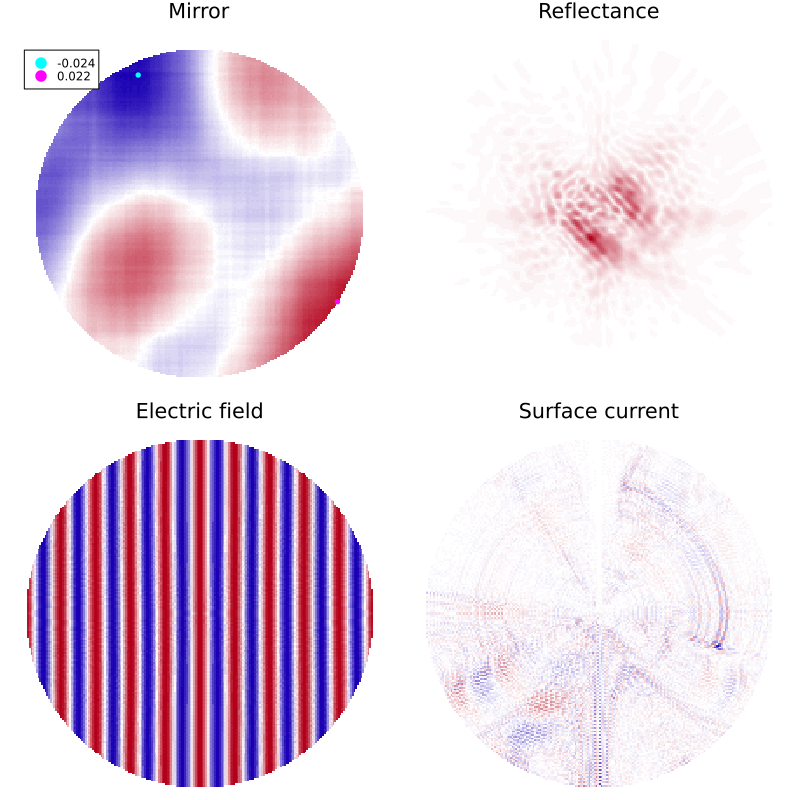
\includegraphics[width=\textwidth]{100-ring-results}}
  \caption[Results with 100 rings]{\label{fig:100_rings}
    Results with 100 rings}
\end{figure}

Using more rings made very little difference. Figure [\ref{fig:30_rings}] shows the results of a simulation with identical parameters, save that 30 rings were used instead of 100.

\begin{figure}
  \centerline{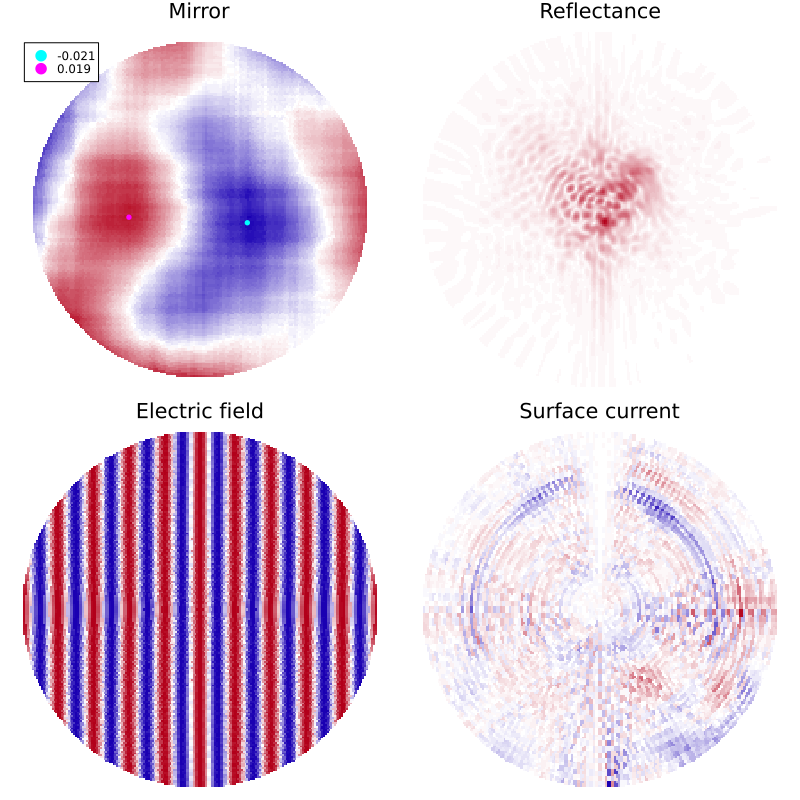
\includegraphics[width=\textwidth]{30-ring-results}}
  \caption[Results with 30 rings]{\label{fig:30_rings}
    Results with 30 rings}
\end{figure}

It seems likely that the results are poor due to the high condition numbers of the impedance matrices. For the simulation mentioned above, the condition numbers were 85.2 billion with 100 rings [\ref{fig:100_rings}] and 1.43 billion with 30 rings [\ref{fig:30_rings}].

%%%%%%%%%%%%%%%%%%%%%%%%%%%%%%%%%%%%%%%%%%%%%%%%%%%%%%%%%%%%%%%%%%%%%%%%%%%%%%%%%%%%%%%%%%%%%%%%%%%%%%%%%%%%%%%%%%%%%%%%





% CONCLUSION %%%%%%%%%%%%%%%%%%%%%%%%%%%%%%%%%%%%%%%%%%%%%%%%%%%%%%%%%%%%%%%%%%%%%%%%%%%%%%%%%%%%%%%%%%%%%%%%%%%%%%%%%%%

\chapter{Conclusion}\label{chap:conclusion}

A program simulating reflectance from a rough conducting surface was built, but proved inaccurate. The code may provide a useful starting point if the model can be tweaked to reduce the condition numbers of the impedance matrices used.

%%%%%%%%%%%%%%%%%%%%%%%%%%%%%%%%%%%%%%%%%%%%%%%%%%%%%%%%%%%%%%%%%%%%%%%%%%%%%%%%%%%%%%%%%%%%%%%%%%%%%%%%%%%%%%%%%%%%%%%%





% APPENDICES %%%%%%%%%%%%%%%%%%%%%%%%%%%%%%%%%%%%%%%%%%%%%%%%%%%%%%%%%%%%%%%%%%%%%%%%%%%%%%%%%%%%%%%%%%%%%%%%%%%%%%%%%%%

\begin{appendices}

  \chapter{Circular Integration}\label{chap:circular_integration}
  
  What follows is Dr. Turley's work, which was foundational for this project and is referenced frequently.
  
  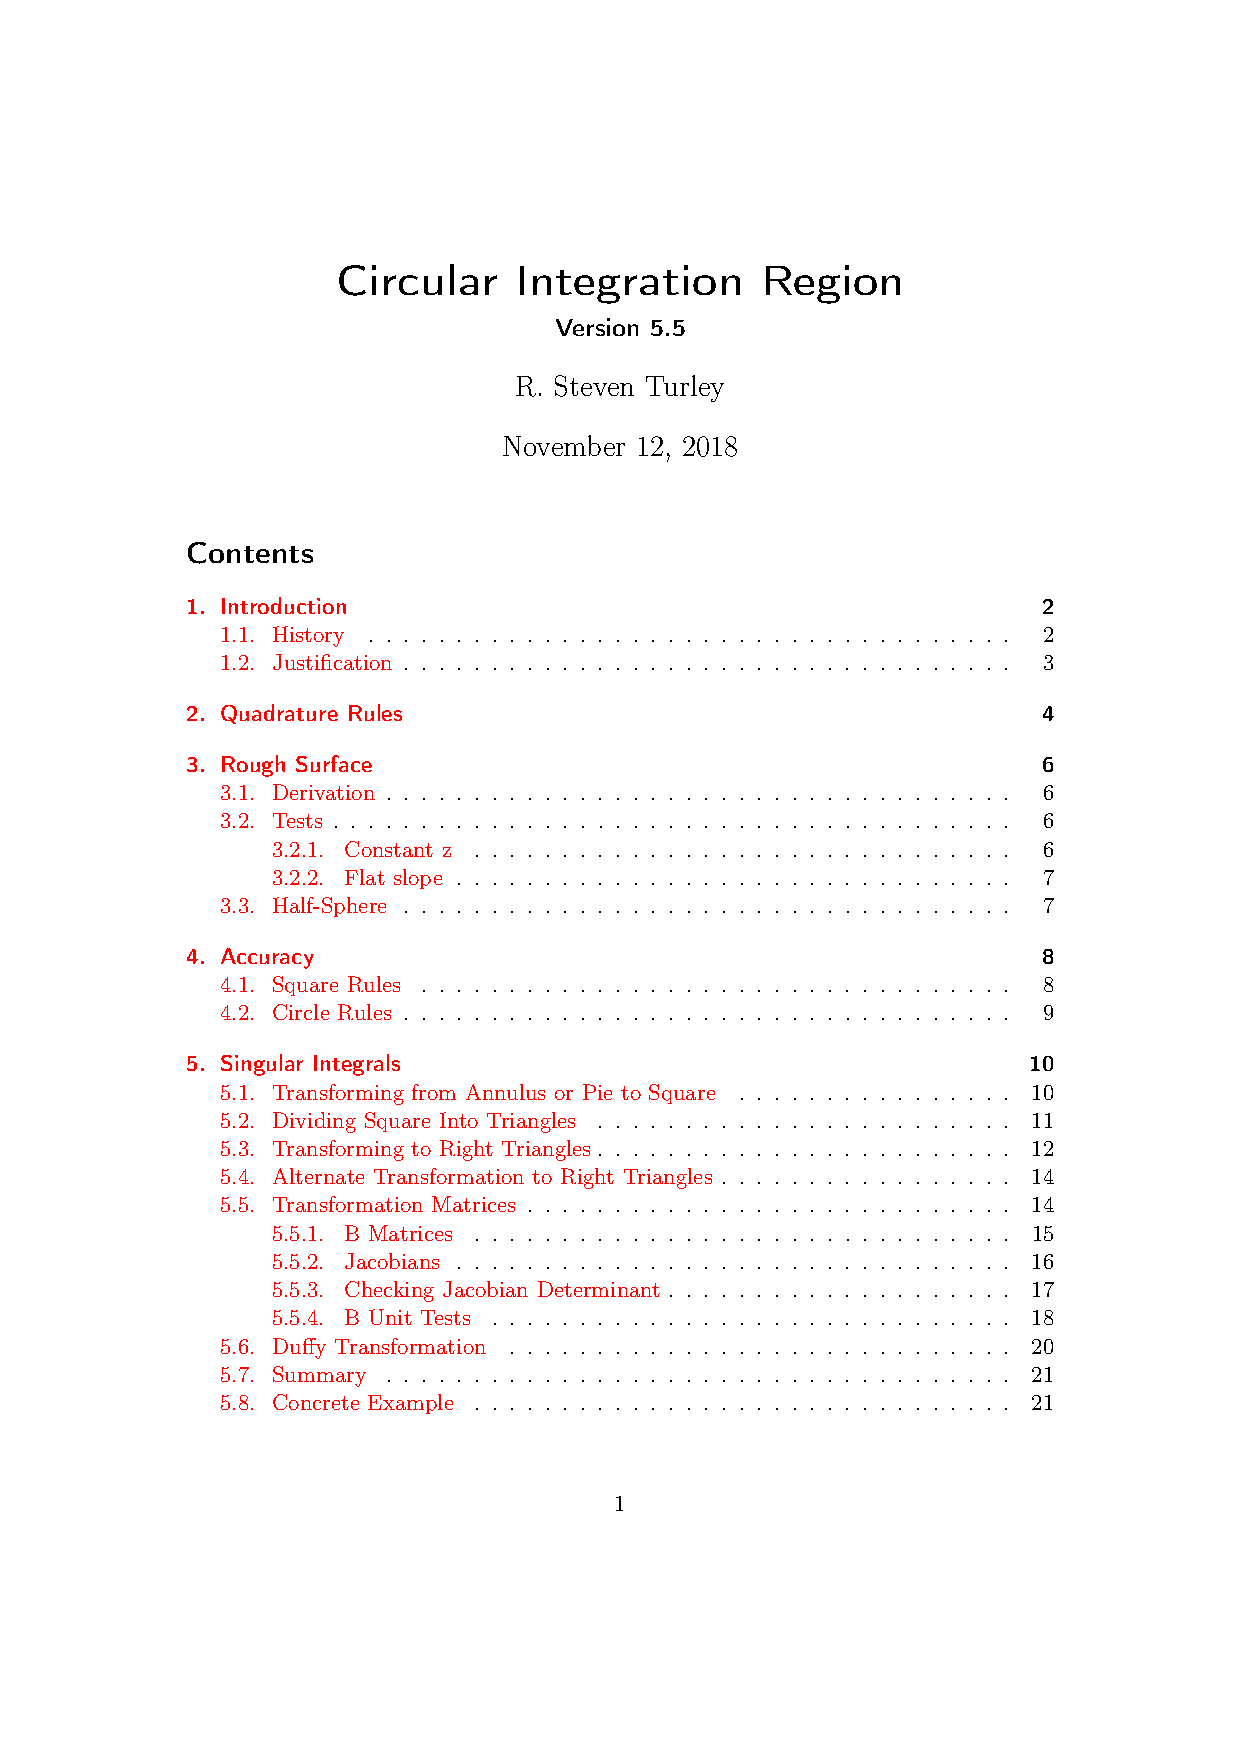
\includepdf[pages=-]{figures/circular-integration.pdf}
  
  
  
  \chapter{Generating Heatmaps}\label{chap:heatmap_code}
  
  Given a \texttt{Reflectance} object \texttt{R}, a heatmap of said reflectance can be generated with:
  
  \begin{minted}{julia}
    heatmap((R.==0).*-max(R...)./2 + R, aspect_ratio=:equal,
                                        colorbar=false,
                                        xticks=false,
                                        yticks=false,
                                        axis=false,
                                        background=false)
  \end{minted}
  
  This was used to generate several of the figures above.
  
  
  
  \chapter{Integral of Equation \ref{eq:integral1}}\label{chap:integral}
  
  Integration was done with Mathematica 13.1.0.
  
  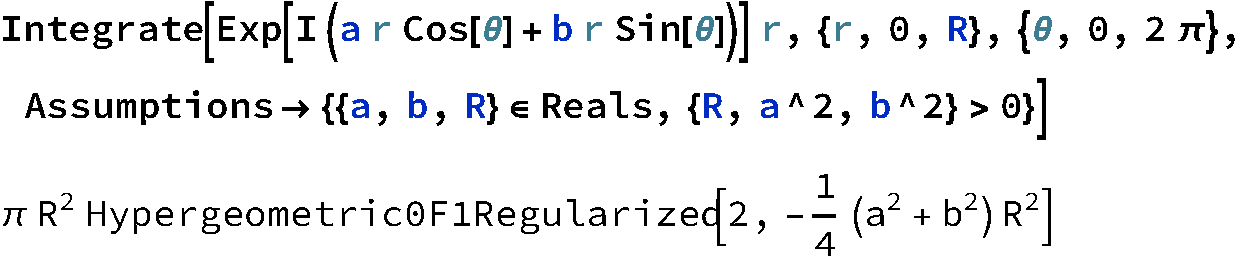
\includegraphics[width=\textwidth]{nasty-integral.pdf}
  
  
  
  \chapter{Simplification of Equation \ref{eq:expected_refl} Given Normal Light Incidence}\label{chap:airy_validation}
  
  Simplification was done with Mathematica 13.1.0.
  
  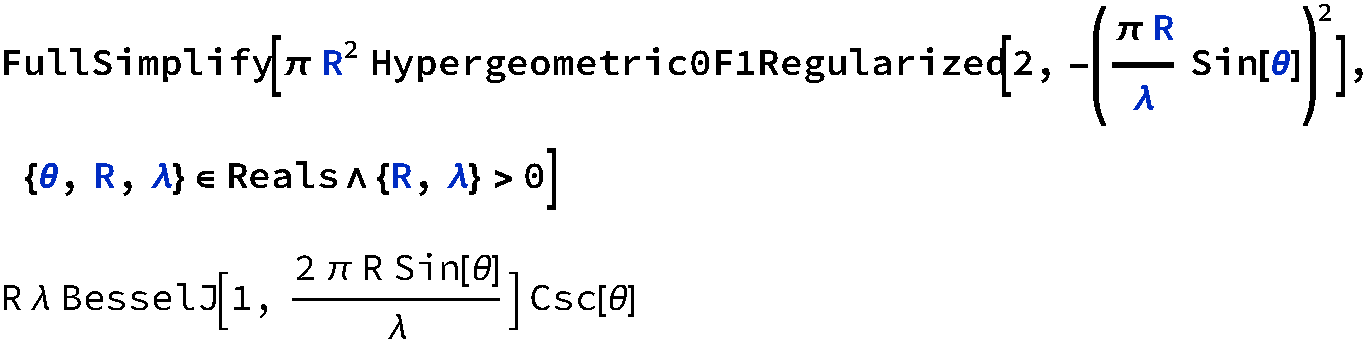
\includegraphics[width=\textwidth]{airy-simplification.pdf}
  
  
  
  \chapter{The Code}\label{chap:julia}
  
  \section{Structure}
  
  \href{https://github.com/mjg0/Mirrors.jl}{Mirrors.jl} is a fully functional Julia package with the following directory structure:
  
  \lstinputlisting[basicstyle=\ttfamily]{code-directory-structure.txt}
  
  These files are included below.
  
  \begin{tiny}
    \input{code.tex}
  \end{tiny}
  
\end{appendices}

%%%%%%%%%%%%%%%%%%%%%%%%%%%%%%%%%%%%%%%%%%%%%%%%%%%%%%%%%%%%%%%%%%%%%%%%%%%%%%%%%%%%%%%%%%%%%%%%%%%%%%%%%%%%%%%%%%%%%%%%





% Make the bibliography.
% Enter your references in the BibTex file "references.bib"
\bibliography{references}

% Make the index
\printindex

\end{document}
